% --------------------------------------
% Document Class
% --------------------------------------
\documentclass[11pt]{article}
% --------------------------------------



% --------------------------------------
% Use Package
% --------------------------------------

% french, english
\usepackage[francais]{babel}

% font, french accent
\usepackage[utf8]{inputenc} 
\usepackage[T1]{fontenc} 

% page layout
\usepackage{geometry}

% hypertext link
\usepackage[pdfpagelabels]{hyperref}

\usepackage{graphicx}
\usepackage{float}
\usepackage{verbatim}
\usepackage{fancyhdr}
\usepackage{amsmath}


% include pdf
\usepackage[final]{pdfpages}


% --------------------------------------



% --------------------------------------
% Page setting
% --------------------------------------
%\pagestyle{empty}
\setlength{\headheight}{15pt}

\setcounter{secnumdepth}{3}
\setcounter{tocdepth}{2}

\makeatletter
\@addtoreset{chapter}{part}
\makeatother 

\hypersetup{         % parametrage des hyperliens
  colorlinks=true,      % colorise les liens
  breaklinks=true,      % permet les retours à la ligne pour les liens trop longs
  urlcolor= blue,       % couleur des hyperliens
  linkcolor= black,     % couleur des liens internes aux documents (index, figures, tableaux, equations,...)
  citecolor= green      % couleur des liens vers les references bibliographiques
}

% --------------------------------------

% --------------------------------------
% Information
% --------------------------------------
\title{Compte-rendu TP2 Rdf : Codage d'un contour}
\author{Elliot VANEGUE et Gaëtan DEFLANDRE}
% --------------------------------------



% --------------------------------------
% Begin content
% --------------------------------------
\begin{document}

  % Set language to english
  \selectlanguage{francais}

  % Start the page counting
  \pagenumbering{arabic}

  \maketitle
  
  \mbox{}
  \newpage
  \clearpage
  
  \section{Introduction}
  Lors de ce TP, nous allons utiliser différents algorithmes permettant de déterminer
  les contours d'une forme afin de connaître les avantages et inconvénients de chacun
  d'eux. Nous étudierons les descripteurs de Fourier, ainsi que l'algorithme
  de la corde.
  
  \section{Descripteurs de Fourier}
  Dans un premier temps nous allons calculer les descripteurs de Fourier. Pour cela
  Nous allons charger un fichier texte et calculer les descripteurs avec la méthode
  fft disponible dans la bibliothèque du langage R. Nous pouvons voir que lorsque
  nous normalisons et que nous inversons les résultats de ce calcul, nous obtenons
  à nouveau la position des points du contour.\\ 
  % TODO comment on le determine
  %On peut voir, suite à ces résultats
  %que le descripteur Z0 est le barycentre 
  
  Nous avons ensuite développé une méthode de filtrage des descripteurs de Fourier dans le
  but d'en éliminer pour rendre le codage d'une forme plus simple à calculer.
  Nous remarquons que moins il y a de descripteur, plus la forme du carré se transforme en cercle.
  Cela se produit, car nous perdons en précision lorsque nous réduisons le nombre de descripteurs.
  
  \begin{figure}[!h]
    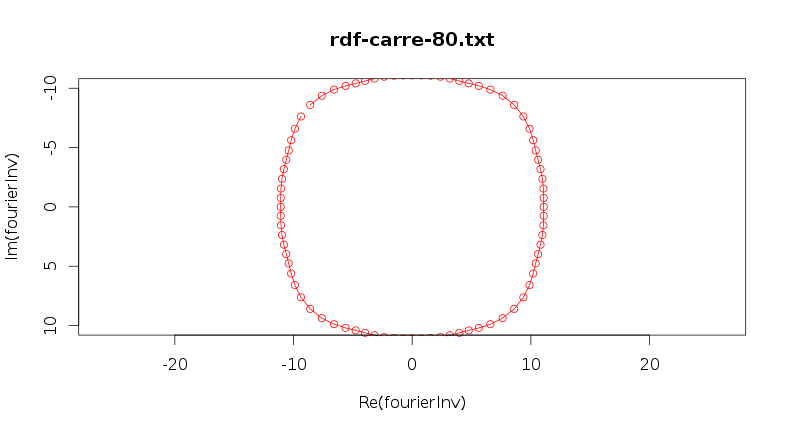
\includegraphics[width=15cm]{../resultat/carre-fourier-20.png}
    \caption{Image du carré avec 80\% des points supprimés}
  \end{figure}
  
  Les descripteurs de Fourier fournissent de bons résultats pour déterminer les contours d'une forme. 
  Cependant, il n'est pas possible de réduire le nombre de calculs, pour une forme rectangulaire, 
  en éliminant des descripteurs.

  \section{Réduction d'une chaîne de contour}
  Nous allons étudier un second algorithme qui est celui de la corde.
  Cet algorithme va tracer des segments qui vont suivre les contours d'une forme. Ces segments 
  devront être le plus proche possible des contours de celle-ci. La distance entre ces segments 
  et les points de la forme sera un paramètre que l'on pourra modifier afin d'avoir le niveau de 
  précision qui convient le mieux. Sur une majorité des formes, plus on demandera une distance petite, 
  plus l'algorithme devra calculer de points.\\ 
  
  
  \begin{figure}[!h]
    \begin{center}
      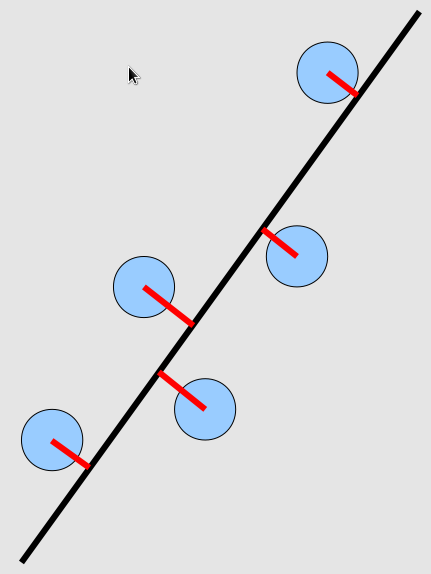
\includegraphics[width=6cm]{corde.png}
    \end{center}
    \caption{Algorithme de la corde}
  \end{figure}
  
  
  Sur l'image ci-dessus les cercles représentent les points d'une forme et la droite correspond
  à un des segments de la corde. Il faut donc calculer la distance entre chaque point et la corde
  afin de déterminer les contours d'une forme.
  Pour calculer cette distance, nous avons utilisé la formule suivante :
  $abs(Im((cont - debut) * Conj(fin - debut))) / Mod(fin - debut)$.
  Cela nous a permis d'obtenir des contours plus ou moins précis en fonction de cette distance.\\
  
  \begin{figure}[!h]
    \begin{center}
      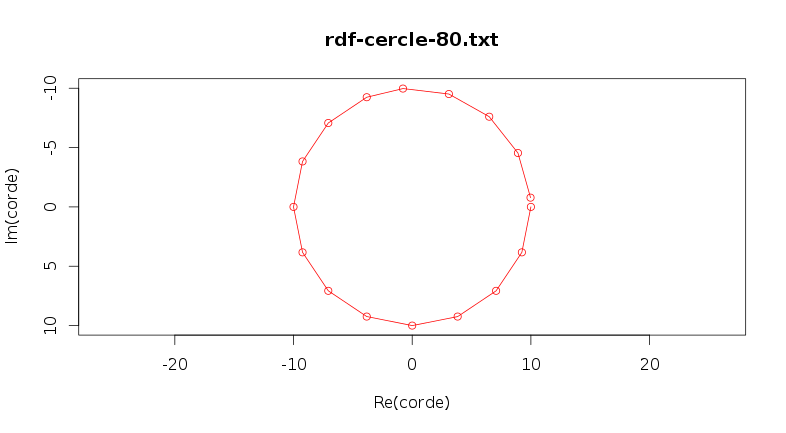
\includegraphics[width=10cm]{../resultat/cercle-corde-5.png}
    \end{center}
    \caption{Image du cercle avec une distance maximum de 0.5 pixels}
  \end{figure}

  \begin{figure}[!h]
    \begin{center}
      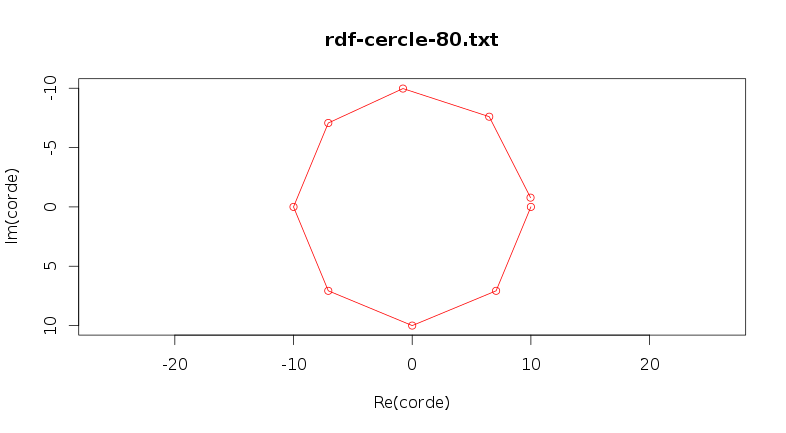
\includegraphics[width=10cm]{../resultat/cercle-corde-10.png}
     \end{center}
    \caption{Image du cercle avec une distance maximum de 1 pixels}
  \end{figure}
  
  \newpage
  
  Nous pouvons voir que cet algorithme reconnaît assez bien la forme du cercle à la condition 
  que la distance entre les points du contour de la forme et la corde soit assez petite. Ce qui 
  implique qu'il faut calculer beaucoup de points pour avoir un résultat satisfaisant.\\
  
  Maintenant que nous savons calculer les descripteurs de Fourier et utiliser l'algorithme
  de la corde nous allons comparer les résultats qu'ils fournissent sur différentes formes.
  
  \section{Comparaison des deux approches}
  Dans la suite de ce rapport, la courbe bleue représentera le tracé des descripteurs de Fourier 
  et la courbe rouge le tracé de l'algorithme de la corde. 
  
  
    \begin{figure}[!h]
      \begin{center}
	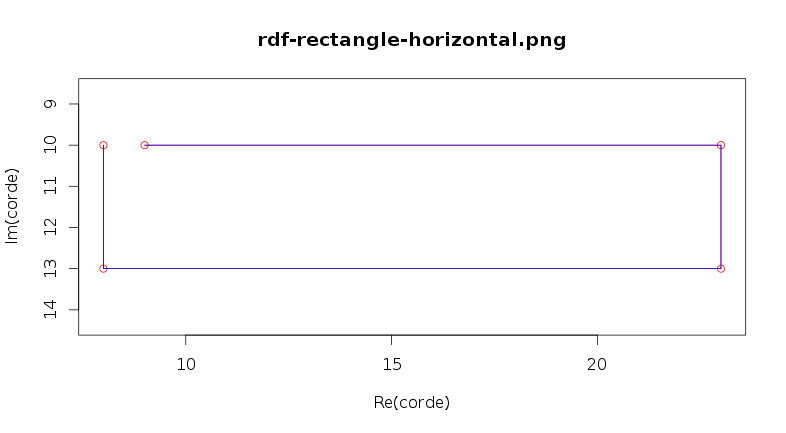
\includegraphics[width=13cm]{../resultat/comp_rect.png}\\
	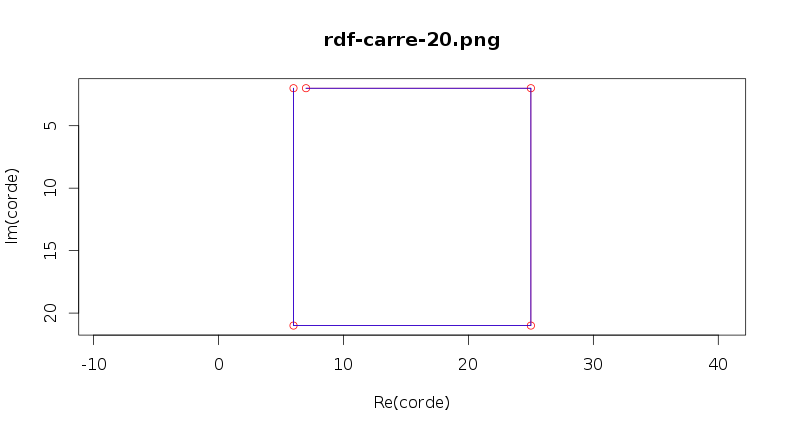
\includegraphics[width=13cm]{../resultat/comp_carre.png}
      \end{center}
      \caption{Comparaison sur le rectangle horizontal et le carré: 100\% de descripteurs gardés et une distance de corde aléatoire}
    \end{figure}
  
  \newpage
  
  Pour le rectangle et le carré, les deux méthodes sont aussi efficaces l'un que l'autre. Cependant, l'algorithme de la corde
  fonctionne très bien avec un minimum de point à calculer.
  De plus, lorsque nous éliminons quelques descripteurs de Fourier, l'algorithme n'est plus capable de
  retrouver la forme, que ce soit pour le rectangle ou le carré.\\
  
  \begin{center}
    \begin{figure}[!h]
      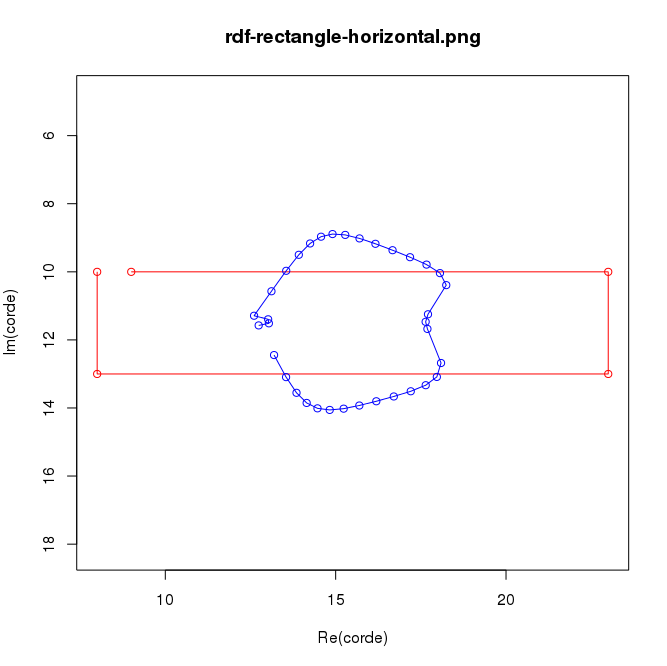
\includegraphics[width=13cm]{../resultat/comp_rate_rect.png}
      \caption{Comparaison sur le rectangle horizontal avec 90\% de descripteurs gardé}
    \end{figure}
  \end{center}
  
  \newpage
  
  Pour le triangle, le calcul des descripteurs de Fourier n'est pas très efficace même si nous gardons
  l'ensemble des descripteurs. L'algorithme de la corde quant à lui a besoin d'une distance minimale de 0.7 pixels pour
  reconnaitre parfaitement le triangle.
  
  \begin{center}
    \begin{figure}[!h]
      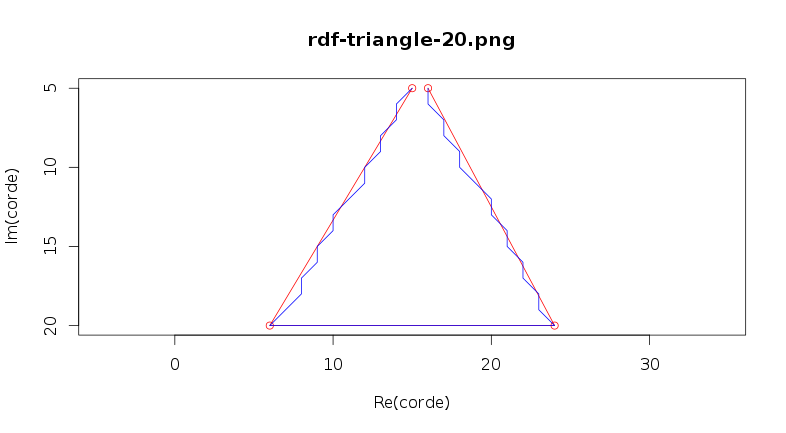
\includegraphics[width=15cm]{../resultat/comp_triangle.png}
      \caption{Comparaison sur le rectangle horizontal avec 90\% de descripteurs gardé}
    \end{figure}
  \end{center}
  
  \newpage
  
  Pour la croix, les observations sont les mêmes que pour le carré et le rectangle. Il faut tous
  les descripteurs de Fourier pour avoir un contour correct et la distance pour l'algorithme de la
  corde n'a pas d'importance.
  
  \begin{center}
    \begin{figure}[!h]
      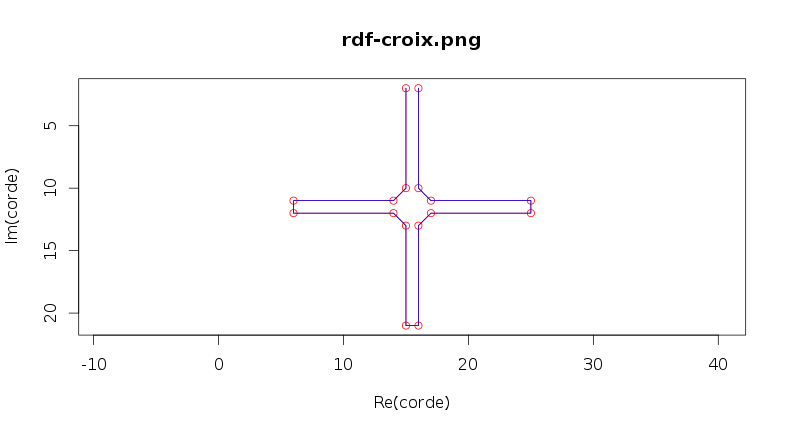
\includegraphics[width=15cm]{../resultat/comp_croix.png}
      \caption{Comparaison sur la croix}
    \end{figure}
  \end{center}
  
  \newpage
  
  Pour la patatoïde, les deux algorithmes sont efficaces, mais la distance pour l'algorithme de 
  la corde fait varier la précision du contour. Pour un contour parfait il faut une distance de 0.1 pixel.
  
  \begin{center}
    \begin{figure}[!h]
      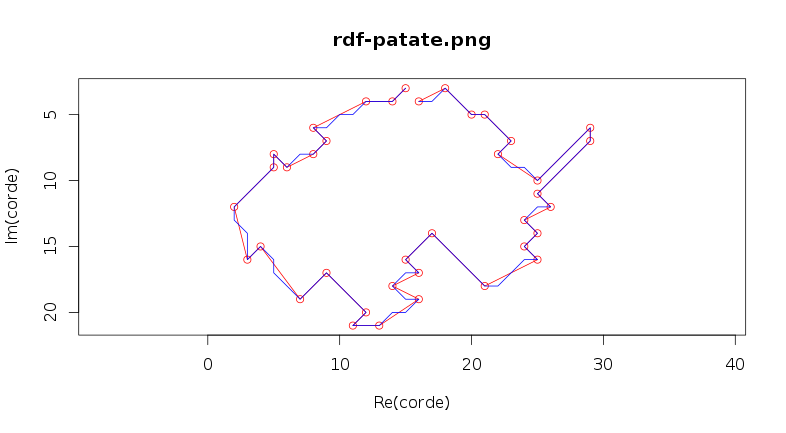
\includegraphics[width=14cm]{../resultat/comp_patate_impreci.png}
      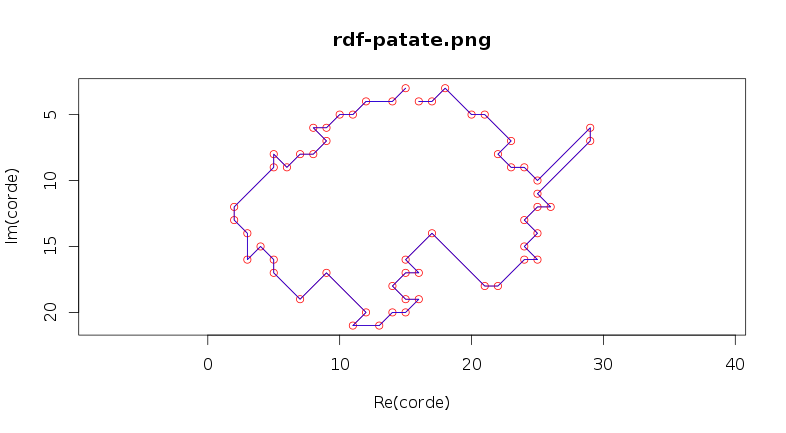
\includegraphics[width=14cm]{../resultat/comp_patate_preci.png}
      \caption{Comparaison sur la patate avec deux niveaux de précision pour l'algorithme de la corde}
    \end{figure}
  \end{center}
  
  \newpage
    
  \section{Conclusion}
  Suite au résultat que nous avons collecté précédemment, on peut voir que les descripteurs de Fourier sont assez 
  efficaces pour des formes circulaires où l'on peut même éliminer des descripteurs pour améliorer les performances 
  de l'algorithme. Pour le reste des formes, il est efficace à condition d'avoir tous ses descripteurs. L'algorithme 
  de la corde est très efficace sur les formes rectangulaires où il a besoin de très peu de points pour obtenir un 
  contour parfait, ce qui rend le contour plus compact. Sur les formes arrondies par contre, il faut que la distance 
  entre la corde et les points de la forme soit très petite pour que le contour soit bien reconnu.\\
  
  Donc l'algorithme de la corde est peut-être plus intéressant que le calcul des descripteurs Fourier, car cette méthode 
  peut-être très efficace avec un minimum de calcul sur certaines formes et il est au moins aussi efficace que la méthode 
  de Fourier sur des formes plus complexes.
  
\end{document}